\documentclass[12pt, t]{beamer}

\usepackage{graphicx}
\usepackage{amsmath}
\usepackage{setspace}
\usepackage{float} 
\usepackage{multido}
\usepackage{multirow}
\usepackage{array}
\usepackage{enumerate}
\usepackage{booktabs}
\usepackage{indentfirst} 
\usepackage[style=mla]{biblatex}
\usepackage{subcaption}
\usepackage{hyperref}
\usepackage{textpos}

\makeatletter
\let\@@magyar@captionfix\relax
\makeatother

\definecolor{Turquoise3}{RGB}{0, 134, 139}
\renewcommand{\emph}[1]{{\color{Turquoise3}\textsl{#1}}}
\newcommand{\C}{\mathbb{C}} \newcommand{\F}{\mathbb{F}} \newcommand{\R}{\mathbb{R}} \newcommand{\Q}{\mathbb{Q}}
\newcommand{\N}{\mathbb{N}}
\newcommand{\myseries}[2]{$#1_1,#1_2,\dots,#1_#2$}
\newcommand{\nullspace}{~\\[15pt]}
\newcommand{\remark}{\textbf{Remark: }}
\newcommand{\scp}[2]{\langle\,#1\,,\,#2\,\rangle} \newcommand{\scpp}{\langle\,\cdot\,,\,\cdot\,\rangle}


\usetheme{Madrid}
\setbeamertemplate{navigation symbols}{}

\addtobeamertemplate{frametitle}{}{
\begin{textblock*}{100mm}(0.85\textwidth,-1cm)

\includegraphics[height=1cm]{logo.png}
\end{textblock*}}

\definecolor{themecolor}{RGB}{25,25,112} 

\usecolortheme[named=themecolor]{structure}

\setbeamertemplate{items}[default]

\hypersetup{
    colorlinks=true,
    linkcolor=themecolor,
    filecolor=themecolor,      
    urlcolor=themecolor,
    citecolor=themecolor,
}

\title{VV285 RC Part II}
\subtitle{\textbf{Elements of Linear Algebra}\\``Linear Algebra!"}
\institute[UM-SJTU JI]{Univerity of Michigan-Shanghai Jiao Tong University Joint Institute}
\author{Yiwen Tu}

\begin{document}

\begin{frame}
    \titlepage
    \begin{center}
        
\includegraphics[height=2cm]{logo2.png}
    \end{center}
\end{frame}
    
\begin{frame}
    \frametitle{Matrices}
    \begin{center}
        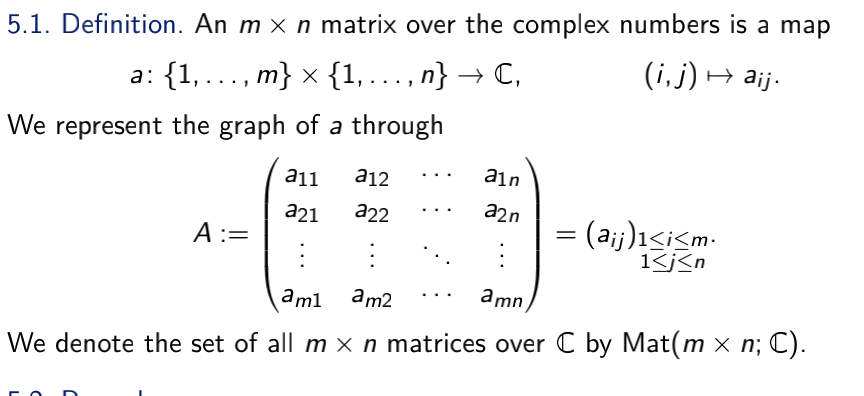
\includegraphics[width=\textwidth]{2}
    \end{center}
\end{frame}

\begin{frame}
    \frametitle{Matrices}
    \begin{center}
        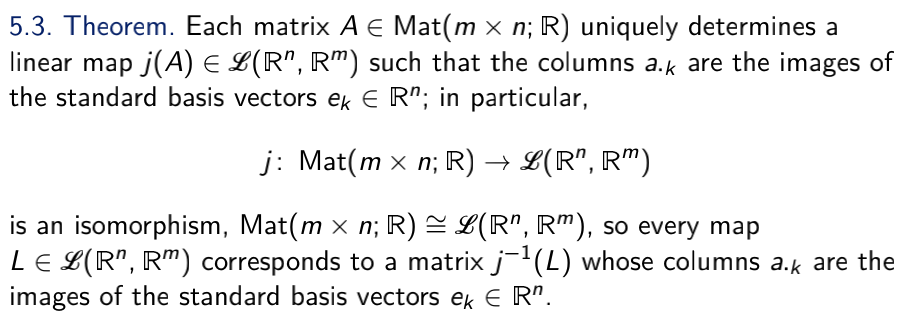
\includegraphics[width=\textwidth]{3}
    \end{center}
\end{frame}

\begin{frame}
    \frametitle{Matrices}
    \begin{center}
        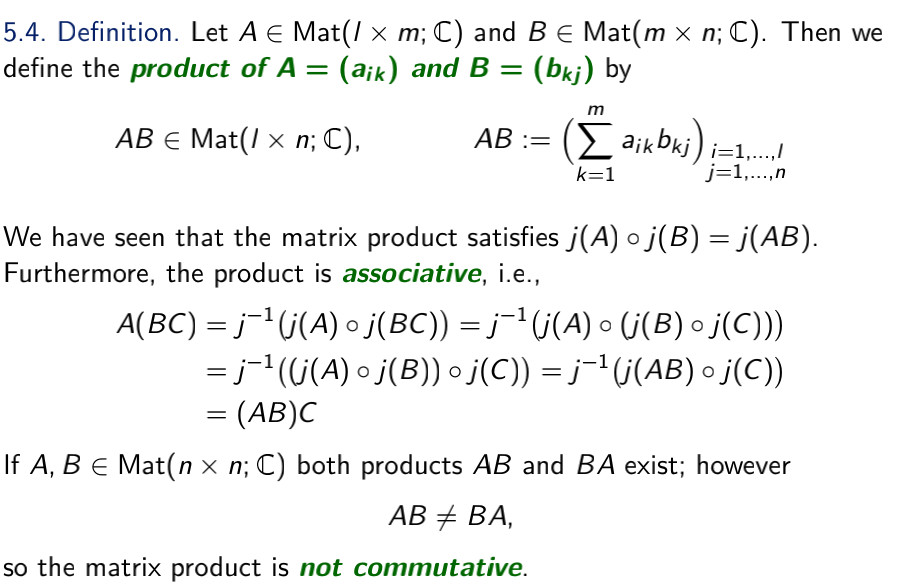
\includegraphics[width=\textwidth]{4}
    \end{center}
\end{frame}

\begin{frame}
    \frametitle{Matrices}
    \begin{center}
        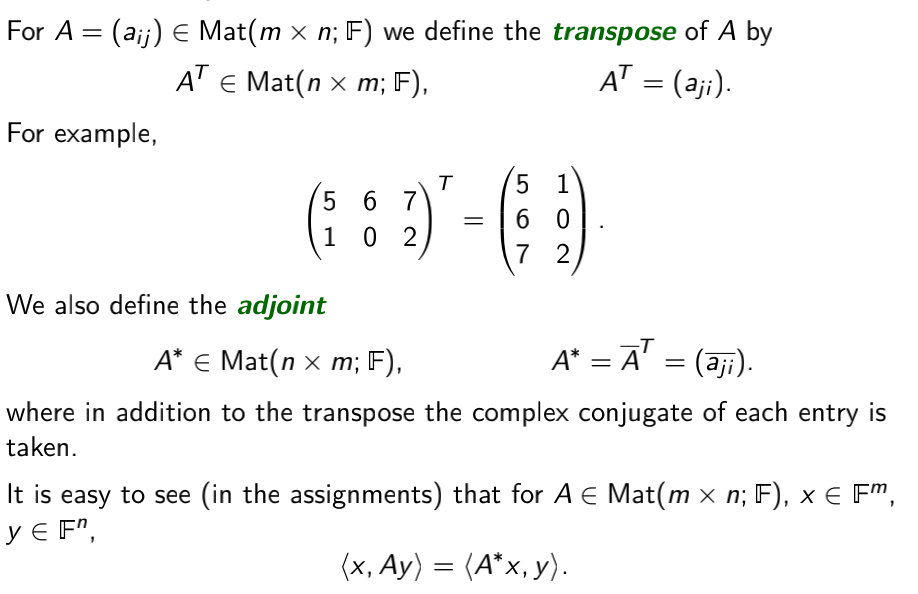
\includegraphics[width=\textwidth]{5}
    \end{center}
\end{frame}
\begin{frame}
    \frametitle{Matrices}
    \begin{center}
        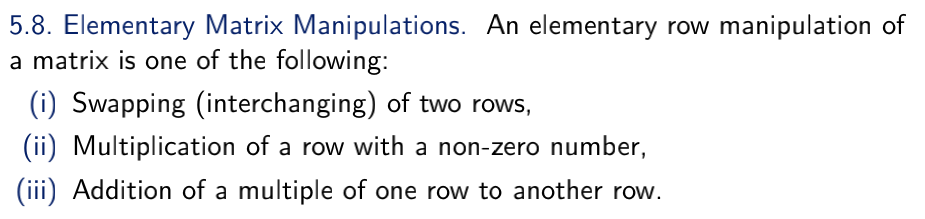
\includegraphics[width=\textwidth]{ele}
    \end{center}
\end{frame}
\begin{frame}
    \frametitle{Matrices}
    \begin{center}
        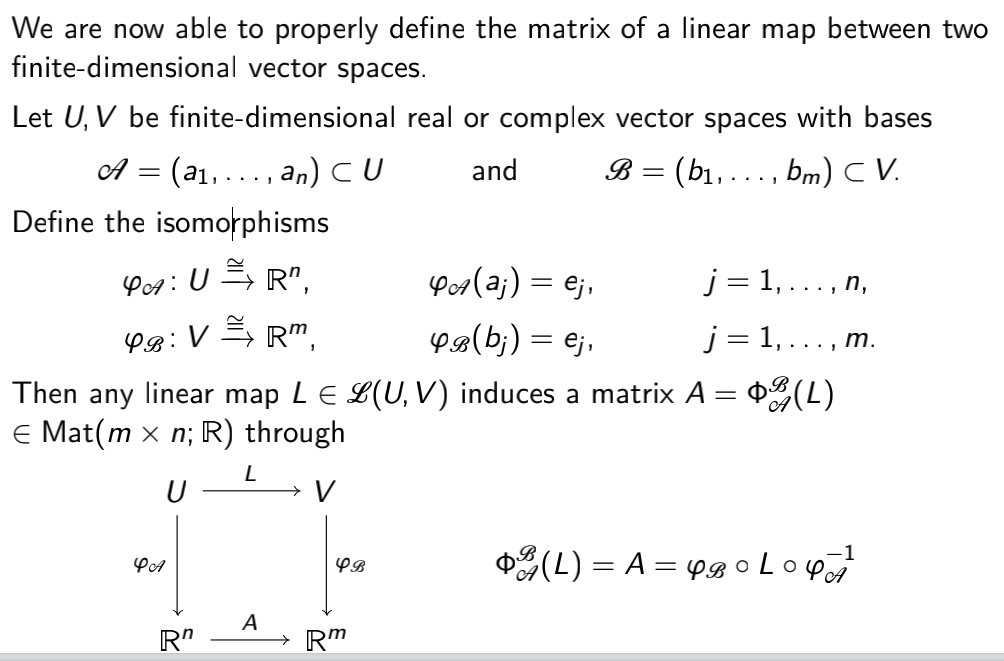
\includegraphics[width=0.9\textwidth]{6}
    \end{center}
\end{frame}
\begin{frame}
    \frametitle{Matrices}
    \begin{center}
        
\includegraphics[width=\textwidth]{7}
    \end{center}
\end{frame}
\begin{frame}
    \frametitle{Matrices}
    \begin{center}
        
\includegraphics[width=\textwidth]{8}
         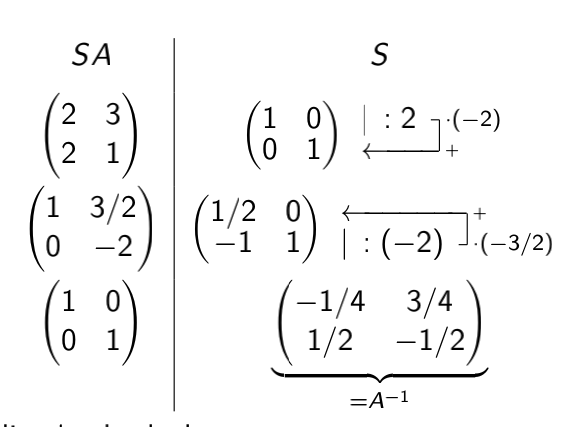
\includegraphics[width=0.65\textwidth]{9}
    \end{center}
\end{frame}
\begin{frame}
    \frametitle{Matrices} 
    \begin{center}
        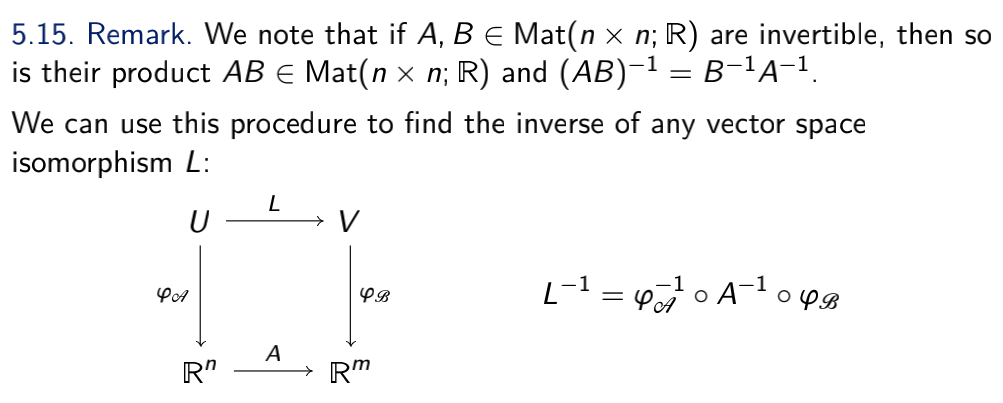
\includegraphics[width=\textwidth]{10}
    \end{center}
\end{frame}
\begin{frame}
    \frametitle{Matrices}
    \begin{center}
        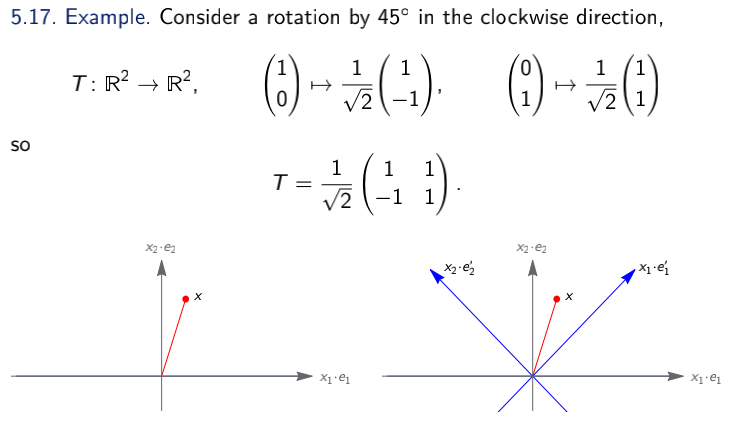
\includegraphics[width=\textwidth]{11}
    \end{center}
\end{frame}
\begin{frame}
    \frametitle{Matrices}
    \begin{center}
        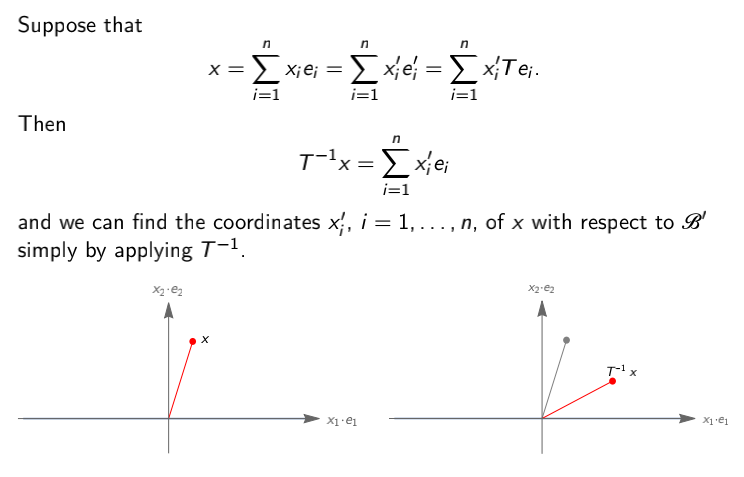
\includegraphics[width=\textwidth]{12}
    \end{center}
\end{frame}

\begin{frame}
    \frametitle{Invertibility of matrices}
Suppose  $||A - I|| < 1$. Show that A is invertible. In particular, show that if 
\[
    A - \alpha  I < ||A||, \alpha \geq ||A||,
\]
then A is invertible.
\end{frame}


\begin{frame}
    \frametitle{Invertibility of matrices}
    This exercise describes the “size” of the set of non-invertible operators.
    Suppose that A is invertible. Show that there is some $\epsilon > 0$ such that for any
    $||A-B|| < \epsilon$ , B is invertible.
\end{frame}


\begin{frame}
    \frametitle{Operator Norm}

    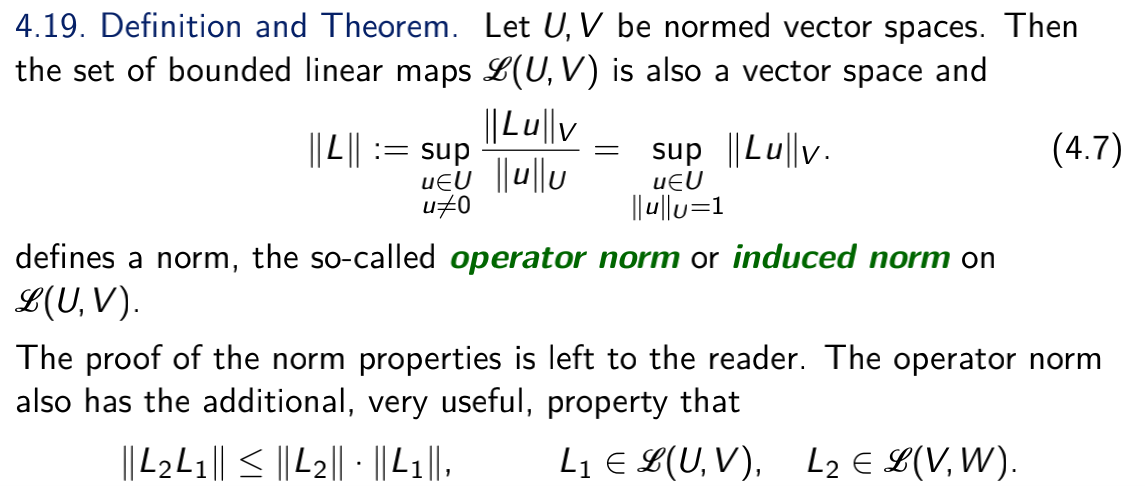
\includegraphics[width=\textwidth]{1}
\end{frame}

\begin{frame}
\frametitle{Adjoint}

\emph{Adjoint} Suppose $T\in L(V,W)$. The adjoint of T is the function $T^{*}: W \rightarrow V$ such that

\[
\langle Tv,w \rangle =\langle v, T^{*}  \rangle
\]

for every $v \in V\textrm{, } w\in W$
\nullspace
The definition makes sense, suppose $T \in L(V,W)\textrm{. fix }w \in W$. Consider the linear functional on V that maps $v \in V \textrm{ to } \langle Tv,w\rangle$; this linear functional depends on T and w. By the Riesz representation Theorem, there exists a unique vector in V such that this linear functional is given by takeing the inner product with it. We call this unique vector $T^{*}w\textrm{. In other words, }T^{*}w$ is the unique vector in V such that the requirement is met for every v in V.
\end{frame}



\begin{frame}
    \frametitle{Properties of the adjoint}
    \begin{itemize}
        \item $(S+T)^{*} =S^{*}+T^{*}$ for all $S,T \in L(V,W)$
        \item $(\lambda T)^{*} =\overline{\lambda} T^{*} $ for all $\lambda \in F$ and $T\in L(V,W)$
        \item $(T^{*})^{*}=T$ for all $T \in L(V,W)$
        \item $I^{*}=I$, where $I$ is the identity operator on V;
        \item $(ST)^{*} =T^{*}S^{*}$ for all $T \in L(V,W)$ and $S \in L(W,U)$ (here $U$ is an inner product space over $F$)
    \end{itemize}
   
\end{frame}

\begin{frame}
    \frametitle{Kernel and Range}
    Suppose $T\in L(V,W)$. then

    \begin{itemize}
        \item $ker T^{*} \bot ran T$
        \item $ker T \bot ran T^{*}$
    \end{itemize}

\end{frame}

\begin{frame}
    \frametitle{Conjugate Transpose}
    The \emph{conjugate transpose} of an m-by-n matrix is the n-by-m matrix obtained by interchanging the rows and columns and then taking tha complex conjugate of each entry.
    Let $T\in L(V,W)$. Suppose $e_1,\cdots e_n$ is an orthonormal basis of V and $f_1, \cdots , f_m$ is an orthonormal basis of W. then
    \[
    M(T^{*}, (f_1,\cdots,f_m), (e_1,\cdots,e_n))  
    \] 
    is the conjugate transpose of 
    \[
    M(T,(e_1,\cdots,e_n), (f_1,\cdots,f_m) )    
    \]
    The proof is not important.
\end{frame}

\begin{frame}
    \frametitle{Self-adjoint operators}
    An operator $T \in L(V)$ is called \emph{self-adjoint} if $T=T^{*}$. In other words, $T\in L(V)$ is self-adjoint if and only if 
    \[
    \langle Tv,w\rangle=\langle v,Tw\rangle    
    \]
    for all $v,w \in V$
    You'll run into more details of self-adjoint operators in VV286!
\end{frame}

\begin{frame}
    \frametitle{$\langle Tv,v \rangle$}
    Try to prove the following two statements!
    \begin{itemize}
        \item Suppose $V$ is a complex inner product space and $T\ in L(V)$. Suppose
        \[
        \langle Tv,v\rangle=0    
        \]
        for all $v \in V$. Then T=0
        \item Suppose $V$ is a complex inner product space and $T\ in L(V)$. Then T is self-adjoint if and only if
        \[
        \langle Tv,v\rangle \in R
        \]
        for all $v \in V$.
    \end{itemize}
\end{frame}

\begin{frame}
    \frametitle{Normal operators}
    An operator on an inner product space is called \emph{normal} if it commutes with its adjoint, or:
    \[
    TT^{*}=T^{*}T    
    \]
    Obviously every self-adjoint operator is normal.
    \nullspace
    An operator $T\in L(V)$ is normal if and only if 
    \[
    ||Tv||=||T^{*}v||    
    \]
\end{frame}

\begin{frame}
    \frametitle{Discussion}
    \vspace{1.5cm}
    \Large
    \centering
    Learn Well\\
    And\\
    Have Fun!\\


\end{frame}

\end{document}